\section{Supplementary Materials}
\label{sec:supplementary}

\subsection{Project Repository}
\label{sec:code}

\subsubsection{Project} \url{https://github.com/piranha-plants-as-charade}.
\subsubsection{Engine (Main Pipeline)} \url{https://github.com/piranha-plants-as-charade/engine/tree/031c9e3091e4f85bd18fd7f51e3f31b7af37c400}.
\subsubsection{Sample Inputs and Outputs + Melody Extraction Tests} \url{https://github.com/piranha-plants-as-charade/results/tree/066bdf375646d9c8fb28b318f0c3aa2c54683533}.
\subsubsection{Cepstrum Analysis Notebook} \url{https://github.com/piranha-plants-as-charade/engine/blob/031c9e3091e4f85bd18fd7f51e3f31b7af37c400/playground/cepstrum_pitch_detection.ipynb}.
\subsubsection{Autocorrelation Analysis Notebook} \url{https://github.com/piranha-plants-as-charade/engine/blob/031c9e3091e4f85bd18fd7f51e3f31b7af37c400/playground/autocorrelation_pitch_detection.ipynb}.

\clearpage
\subsection{Transcription of the Melody Extraction Outputs for the Same Melody With Various Timbres}
\label{sec:sheet_music_melody}

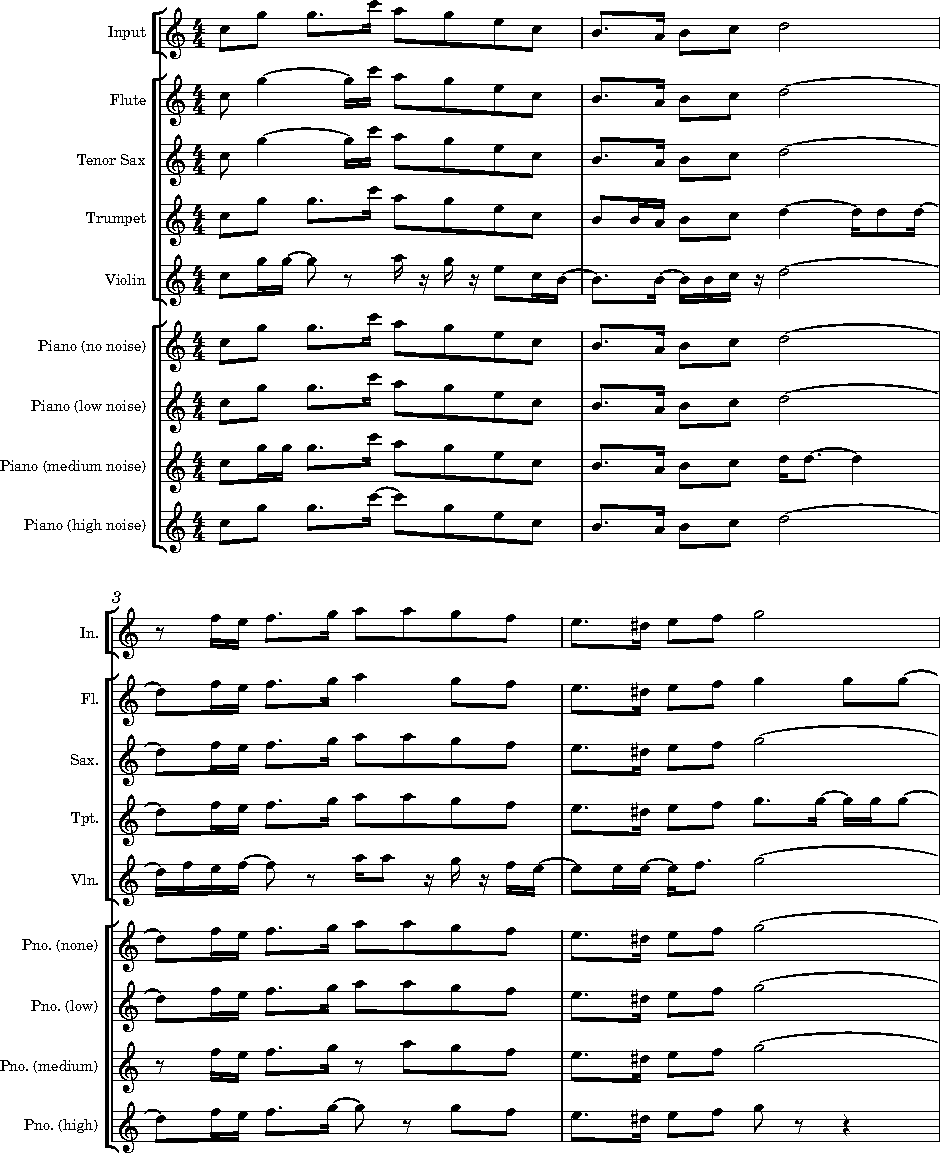
\includegraphics[page=1, width=\linewidth]{materials/piranha_melody.pdf}
\clearpage

\includegraphics[page=2, width=\linewidth]{materials/piranha_melody.pdf}
\clearpage

\clearpage
\subsection{Transcription of the Original and Generated Chord Progression for an Excerpt From ``Piranha Plants on Parade''}
\label{sec:sheet_music_melody}

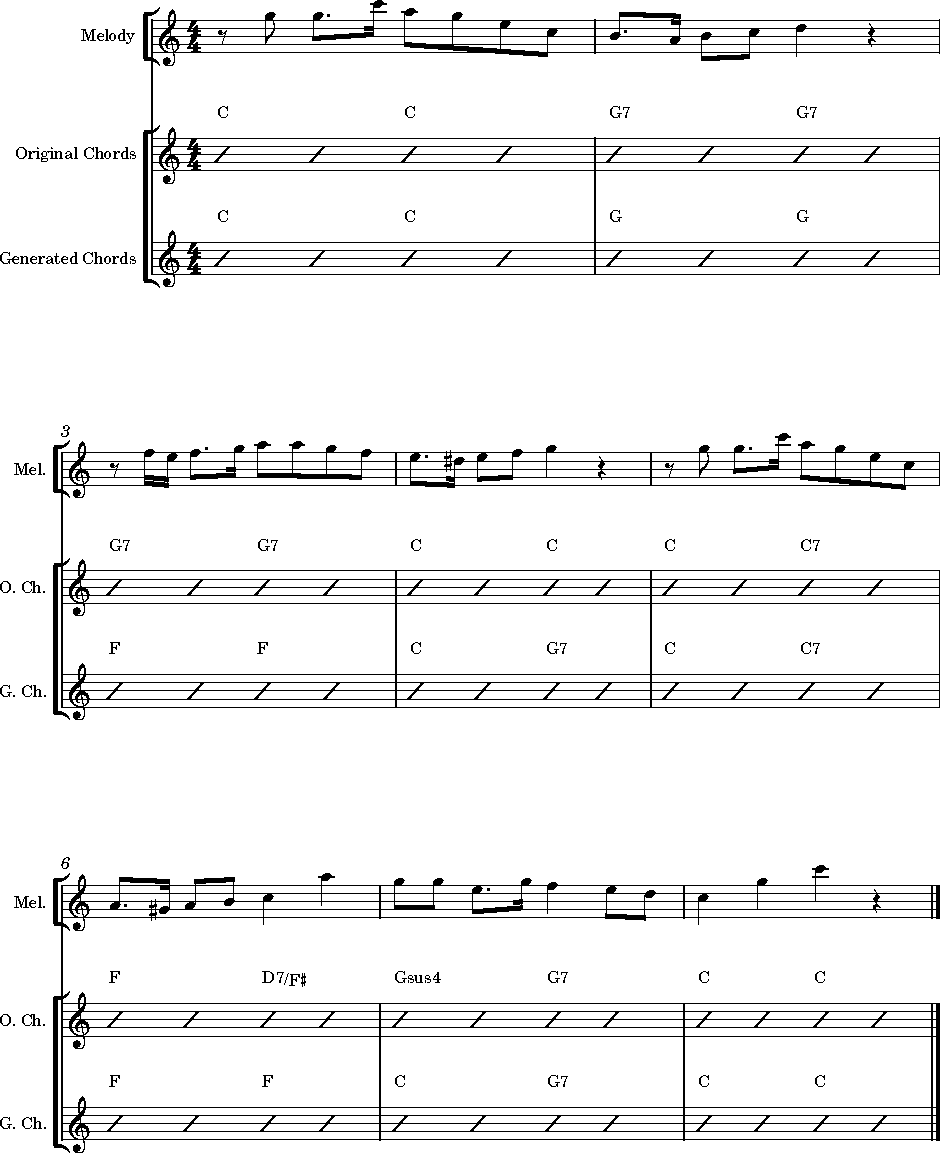
\includegraphics[page=1, width=\linewidth]{materials/piranha_chords.pdf}
\clearpage

% \includegraphics[page=2, width=\linewidth]{materials/piranha_melody.pdf}
% \clearpage

% \clearpage
% \subsection{Transcription of Generated ``Piranha Plants as Parade''}
% \label{sec:sheet_music_generated}

% 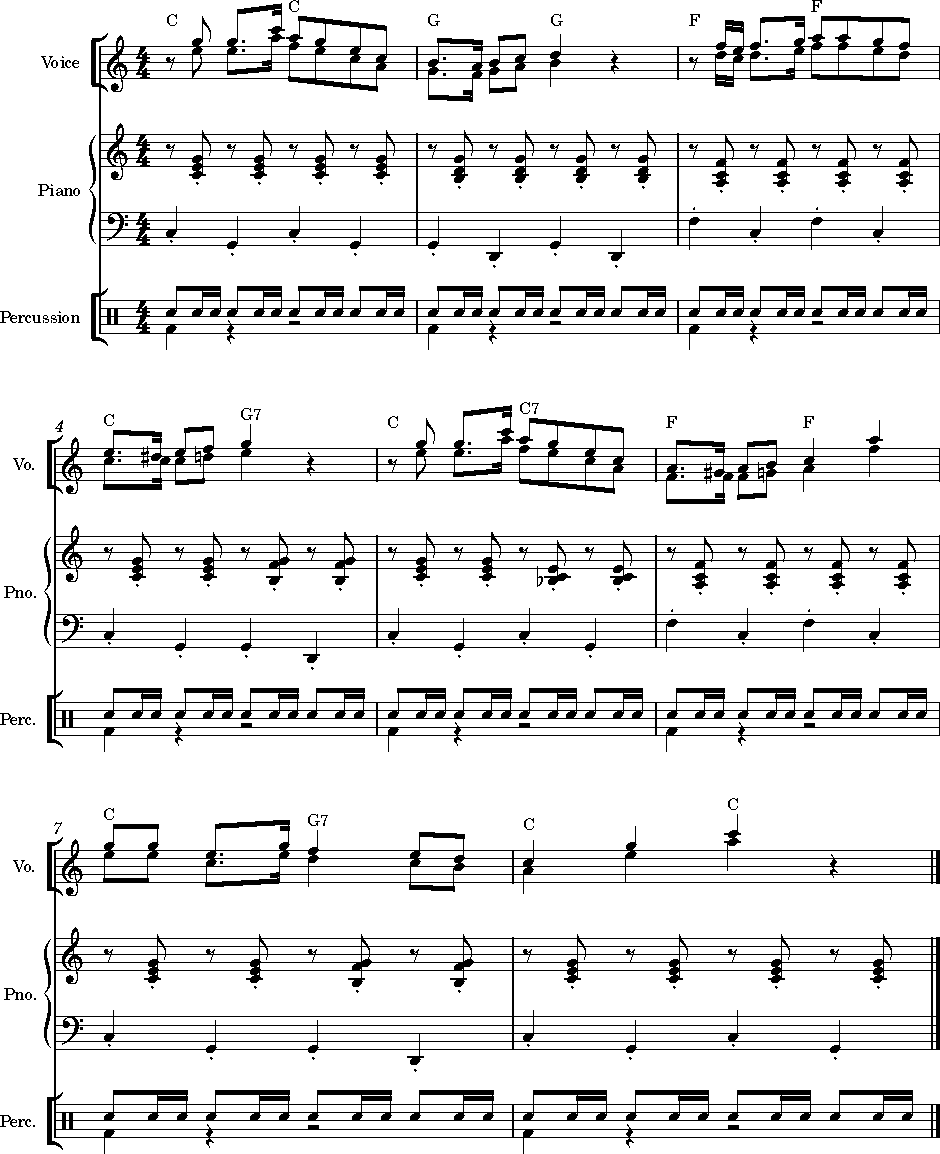
\includegraphics[page=1, width=\linewidth]{materials/piranha_generated.pdf}
% \clearpage

% \clearpage
% \subsection{Transcription of Original ``Piranha Plants on Parade''}
% \label{sec:sheet_music_original}

% This transcription is a simplification of ``Piranha Plants on Parade''. It has been transposed to the key of C Major to simplify comparisons with the outputs from Piranha Plants as Charade.

% 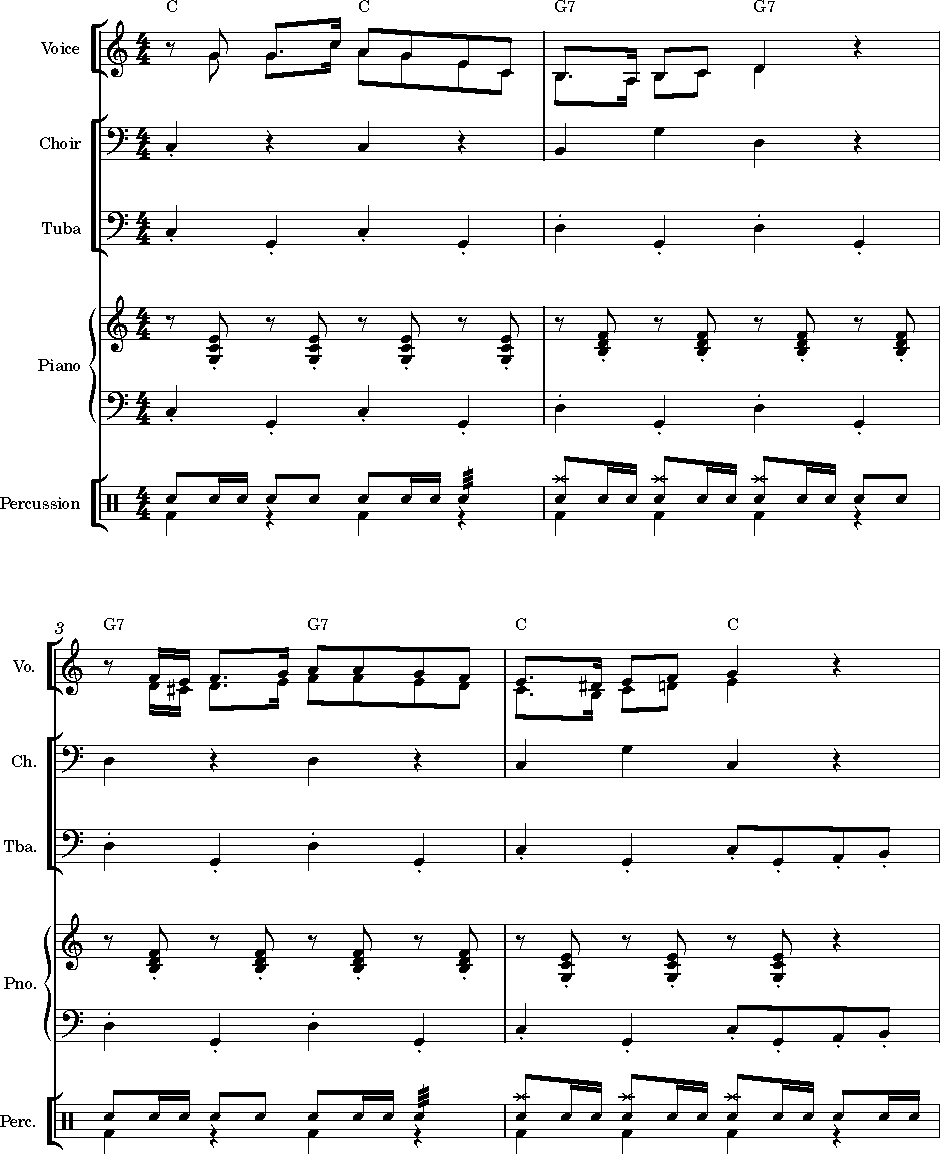
\includegraphics[page=1, width=\linewidth]{materials/piranha_original.pdf}
% \clearpage

% \includegraphics[page=2, width=\linewidth]{materials/piranha_original.pdf}
% \clearpage